\documentclass{article}
\makeatletter
\renewcommand{\fnum@figure}{Εικόνα \thefigure}
\makeatother
\usepackage[greek, english]{babel}
\usepackage{alphabeta}
\usepackage{atbegshi, picture}
\usepackage[letterpaper,top=2cm,bottom=2cm,left=3cm,right=3cm,marginparwidth=1.75cm]{geometry}
\usepackage{amsmath}
\usepackage{graphicx}
\usepackage[colorlinks=true, allcolors=blue]{hyperref}
\usepackage[utf8]{inputenc}
\usepackage{indentfirst}
\usepackage[table]{xcolor}
\usepackage{hyperref} 
 \hypersetup{ 
     colorlinks=true, 
     linkcolor=blue, 
     filecolor=blue, 
     citecolor = black,       
     urlcolor=black, 
     } 

\addto\captionsenglish{
  \renewcommand{\contentsname}
    {Περιεχόμενα}
}

\begin{document}

\begin{titlepage}
   \begin{center}
       \vspace*{1cm}

       \textbf{\huge Team Plan}

       \vspace{0.5cm}
        Τεχνολογία Λογισμικού
            
       \vspace{1cm}

       \textbf{Κούρου Αγγελική\\Βλαχογιάννης Δημήτρης}
       
       \begin{figure}[!htb]
        \centering
        \includegraphics[width=0.5\textwidth]{905e4125666e44b594d9bd286a1d1b61.png}
        \end{figure}
        
        \vspace{0.5cm}
        
        \begin{figure}[!htb]
        \centering
        \includegraphics[width=0.5\textwidth]{up_2017_logo_en.jpg}
        \end{figure}


       \vfill
            
       Τεχνικό Κείμενο για την Τεχνολογία Λογισμικού\\
            
       \vspace{0.5cm}
            
        CEID, ECE \\
       University of Patras\\
            
   \end{center}
\end{titlepage}



\noindent Η ομάδα μας

\begin{enumerate}
  \item Βεργίνης Δημήτριος, ΑΜ: 1066634 , ECE
  \item Βλαχογιάννης Δημήτριος, ΑΜ: 1067371, CEID
  \item Κούρου Αγγελική, ΑΜ: 1067499 , CEID
  \item Μητροπούλου Αικατερίνα - Quality Manager, ΑΜ: 1067409, CEID
  \item Στεφανίδης Μάριος - Project Manager, ΑΜ:1067458, CEID
\end{enumerate}

{
  \hypersetup{linkcolor=black}
  \tableofcontents
}

\section{Εισαγωγή}
   
Στο παρόν τεχνικό κείμενο παρουσιάζεται ο τρόπος χειρισμού του έργου \textbf{Medic World} στο πλαίσιο του μαθήματος "Τεχνολογία Λογισμικού". Αρχικά θα δοθεί μια σύντομη επισκόπηση της ομάδας και στη συνέχεια θα αναλυθούν οι τρόποι και τα εργαλεία υλοποίησης της εργασίας καθώς και θα δοθούν τα διαγράμματα Gannt και Pert που αφορούν τον χρονοπρογραμματισμό της. 
 
 \textbf{Σημείωση:} Όπου υπάρχει η ένδειξη (*) σημαίνει πως το συγκεκριμένο κείμενο αφορά την έκδοση v0.2 του τεχνικού κειμένου Team-Plan.
 
\subsection{Ομάδα Υλοποίησης}

Για την σύσταση της ομάδας επιλέχθηκαν τα παραπάνω πέντε άτομα λαμβάνοντας υπόψιν τις δυνατότητες του καθενός και με ποιον τρόπο αυτές μπορούν να συνεισφέρουν σε μια ομάλη συνεργασία και στην ολοκλήρωση του έργου μας. Ξεκινώντας με τον Project Manager, Στεφανίδη Μάριο, ο οποίος με την οργανωτικότητα, τη σχολαστικότητα και τη συνέπειά του βοηθάει στον καλύτερο συντονισμό και την αποτελεσματική λειτουργία της ομάδας. Ως Quality Manager ορίστηκε η Μητροπούλου Αικατερίνα , η οποία ούσα ένα εργατικό, υπομονετικό και επικοινωνιακό άτομο διαχειρίζεται την εικόνα των εργασιών με σεβασμό απέναντι στους δημιουργούς τους.
\newline \par

Όσον αφορά στα Hard Skills της ομάδας φροντίσαμε τα μέλη που την απαρτίζουν να προσφέρουν το καθένα και κάτι διαφορετικό. Ο Βεργίνης Δημήτριος, θεωρούμε ότι θα διαδραματίσει σημαντικό ρόλο στην ανάπτυξη του κώδικα του \textbf{Medic World} με τις γνώσεις που διαθέτει στη γλώσσα \emph{Python}, ενώ παράλληλα φέρνει μια νέα οπτική εξαιτίας των σπουδών του στο τΗΜΤΥ. Ο Βλαχογιάννης Δημήτριος, έχοντας πολύπλευρες γνώσεις και εμπειρία στο κομμάτι του προγραμματισμού, θα βοηθήσει τα υπόλοιπα μέλη  που ενδεχομένως δεν είναι τόσο εξοικειωμένα στην συγγραφή κώδικα ενώ η εφευρετικότητά του θα έχει ως αποτέλεσμα να παρέχει γρήγορα λύσεις στα πιθανά προβλήματα που θα προκύψουν στην διαδικασία ανάπτυξης του λογισμικού. Η Κούρου Αγγελική έχοντας ως κύριο ενδιαφέρον την ενασχόληση με το υλικό, θα βοηθήσει αφενός στην βέλτιστη αξιοποίηση του και αφετέρου τα υπόλοιπα μέλη να κατανοήσουν την καλύτερη σύνδεση και επικοινωνία του με το λογισμικό. Ακόμα, θα προσθέσει μια νέα οπτική στην ανάπτυξη του \textbf{Medic World}, αν λάβουμε υπόψιν μας πως τα υπόλοιπα μέλη ασχολούνται κυρίως με το κομμάτι του προγραμματισμού. Τέλος, ανεξάρτητα από τις προγραμματιστικές τους γνώσεις, ο Στεφανίδης Μάριος και η Μητροπούλου Αικατερίνα, είναι εξοικειωμένοι με τους κανόνες του UX Design.

\subsection{Εργαλεία Υλοποίησης}

Για την υλοποίηση των επιμέρους διεργασιών του \textbf{Medic World} χρησιμοποιήθηκε μια πληθώρα εργαλείων όπως φαίνεται παρακάτω.


\begin{itemize}
    \item Γλώσσες Προγραμματισμού: Python, SQL
    \item Περιβάλλοντα Ανάπτυξης: PyCharm, Visual Studio Code, QtDesigner, MariaDB
    \item Πλατφόρμες Επικοινωνίας: Discord, Githhub (Issues \& Commits), e-mail
    \item Διαγράμματα Gantt: \underline{\href{https://www.monday.com}{Monday}}
    \item Διαγράμματα Gantt Ανθρώπινου Δυναμικού: \underline{\href{https://microsoft-excel.en.softonic.com/}{Microsoft Excel}}
    \item Διαγράμματα Pert,ER: \underline{\href{https://lucid.app}{Lucidchart}}
    \item Επεξεργασία Τεχνικών Κειμένων: \underline{\href{https://www.overleaf.com}{Overleaf}}
    \item Mock-up Screens: \underline{\href{https://www.figma.com}{Figma}}
    \item Version Control: \underline{\href{https://github.com/mstephanidhs/Software-Engineering}{Github}}
    \item Database Design: \underline{\href{www.dbdesigner.net}{DBDesigner}}
    \item Διαγράμματα Περιπτώσεων Χρήσης: \underline{\href{https://staruml.io/download}{StarUML}}

\end{itemize}

\vspace{0.3cm}

\textbf{Σημείωση:} Το link του Github οδηγεί στη σελίδα της ομάδας μας.
 

\subsection{Μέθοδος Ανάπτυξης Λογισμικού}

(*) Έπειτα από αναλυτική έρευνα των διαφόρων μεθόδων ανάπτυξης λογισμικού, η ομάδα μας περιό-\\ρισε τις επιλογές της στις μεθόδους \textbf{Kanban} και \textbf{Scrum}. Εν τέλει, ύστερα από συζήτηση με όλα τα μέλη της ομάδας και συγκεντρωτική ψηφοφορία, αποφασίστηκε πως κατάλληλη μέθοδος είναι η Scrum για διάφορους λόγους. \newline \par

Αρχικά, θεωρήσαμε πως είναι πιο ευκόλα υλοποιήσιμη για μια νεοσύστατη ομάδα που ασχολείται πρώτη φορά με την ανάπτυξη λογισμικού, έχοντας στη διάθεση της περιορισμένο χρόνο και αυστηρές προθεσμίες παράδοσης. Επίσης, επιτυγχάνεται καλύτερος συντονισμός και οργάνωση, αν λάβουμε υπόψιν πως κάθε sprint cycle αντιστοιχεί στο παραδοτέο που πρέπει να υποβληθεί κάθε φορά (ανά δύο εβδομάδες), ενώ η διαδικασία του planning γίνεται πριν την έναρξη του sprint cycle. Ακόμα, όπως είναι προφανές, στο τέλος κάθε sprint cycle θα πραγματοποιείται αξιολόγηση της δουλειάς που έχει γίνει από τα μέλη της ομάδας σύμφωνα και με όσα που έχουν ειπωθεί στο μάθημα από τους καθηγητές αλλά και από τις απορίες των υπόλοιπων συμφοιτητών μας. Τέλος, στη μέθοδο Scrum οι συναντήσεις πρέπει να είναι καθημερινές, στόχος που θα προσπαθήσουμε να επιτύχουμε για την καλύτερη επικοινωνία και οργάνωση της ομάδας, ωστόσο αυτό θα εξαρτηθεί από την πρόοδο του κάθε task και το πρόγραμμα των μελών. Ωστόσο, επειδή κατανοούμε πόσο σημαντικές είναι οι παραπάνω συναντήσεις, μιας και κατά τη διάρκεια αυτών μπορεί να γίνει περιγραφή της προόδου από την προηγούμενη συνάντηση, να αναφερθούν προβλήματα που έχουν προκύψει καθώς και να αποφασιστεί τι πρέπει να γίνει αμέσως μετά, ο Project Manager θα προσπαθήσει να οργανώνει και ατομικές συναντήσεις πέρα από ομαδικές, με τα μέλη της ομάδας που έχουν αναλάβει το κάθε τεχνικό κείμενο ανά παραδοτέο. \newline \par

Σχετικά με τους ρόλους που περιλαμβάνει η μεθοδολογία Scrum, θα ισχύσουν τα παρακάτω για την δική μας ομάδα:

\begin{itemize}
  \item Scrum Master (στην δική μας περίτπωση Project Manager): Είναι αυτός που θα συντονίζει την ομάδα, θα αναθέτει τις εργασίες και θα επιβλέπει την πρόοδό τους κλπ
  \item Team Members: Αποτελούν το ανθρώπινο δυναμικό της ομάδας
  \item Product Owner: Δεν κρίνουμε πως είναι απαραίτητος ο συγκεκριμένος ρόλος σύμφωνα με τις τρέχουσες συνθήκες αλλά θα μπορούσε να θεωρηθεί πως το αναλαμβάνουν κατά κάποιον τρόπο οι καθηγητές του μαθήματος "Τεχνολογία Λογισμικού"
  \item Quality Manager (ρόλος που δεν περιέχει η μεθοδολογία Scrum αλλά θα χρησιμοποιήσουμε εμείς): Είναι υπεύθυνος για την ποιότητα των αναφορών και της δουλειάς που γίνεται από τα μέλη της ομάδας
\end{itemize}

Σχετικά με τον διαμοιρασμό των tasks ανά παραδοτέο, πριν ξεκινήσει κάθε sprint cycle, η ομάδα θα συναντιέται και όλα τα μέλη μαζί, έπειτα από συζήτηση, θα αποφασίζουν τις αρμοδιότητες που θα αναλάβει ο καθένας. Ώστοσο, ο Project Manager γνωρίζοντας τις ικανότητες (soft \& hard skills) του κάθε μέλους της ομάδας, μπορεί να υποδεικνύει έμμεσα τις εργασίες που θα αναλάβει ο καθένας αλλά και τα μέλη με τα οποία μπορεί να συνεργαστεί από την υπόλοιπη ομάδα επιτυχάνοντας κατά αυτό τον τρόπο την καλύτερη διαχείριση του ανθρώπινου δυναμικού που διαθέτει. Τέλος, καθίσταται σαφές πως στην περίπτωση διενέξεων ή εντάσεων ανάμεσα σε μέλη της ομάδας, ο Project Manager είναι αυτός που οφείλει να διαχειριστεί την κατάσταση.

\section{Διαγράμματα χρονοπρογραμματισμού}

Παρακάτω παρουσιάζονται τα διαγράμματα χρονοπρογραμματισμού Gantt και Pert Charts.

Για τα ορόσημα του έργου ισχύουν τα εξής:
\begin{itemize}
    \item Το πρώτο ορόσημο αφορά την τελική και αναλυτική περιγραφή του \textbf{Medic World}, συνοδευόμενη από τα αντίστοιχα mock-up screens επιδεικνύοντας τις βασικές λειτουργίες του.
    \item Το δεύτερο ορόσημο σχετίζεται με την ολοκλήρωση των Use-Cases, κάποια εκ των οποίων θα υλοποιηθούν σε κώδικα.
    \item Το τρίτο ορόσημο αφορά την πρώτη ολοκληρωμένη έκδοση του κώδικα και τον έλεγχο της λευτουργικότητας του μέσω των Test-Cases.
    \item Το τελευταίο ορόσημο σχετίζεται με την περάτωση του έργου και την παράδοση των τελευταίων εκδόσεων των τεχνικών κειμένων και του κώδικα. 
\end{itemize}

\subsection{Διαγράμματα Pert}

Τα Pert flowcharts που αφορούν τα παραδοτέα της εργασίας παρουσιάζονται παρακάτω. Για περαιτέρω βοήθεια στην κατανόηση πρέπει να γίνουν οι εξής διευκρινίσεις:

\begin{itemize}
  \item Με κόκκινο βέλος συμβολίζεται το κρίσιμο μονοπάτι του έργου, οποιαδήποτε καθυστέρηση του οποίου θα οδηγήσει σε καθυστέρηση όλου του έργου
  \item Οι κίτρινοι ρόμβοι συμβολίζουν τα milestones, επομένως στην προκειμένη περίπτωση τις ολοκληρωμένες παραδόσεις της εργασίας.
\end{itemize}

\newpage

\begin{figure}[!htb]
\centering
\includegraphics[width=1\textwidth]{TeamPert1.png}
\caption{\label{fig:Pert1} Παραδοτέο 1$^o$}
\end{figure}

\begin{figure}[!htb]
\centering
\includegraphics[width=1\textwidth]{TeamPert2.png}
\caption{\label{fig:Pert2} Παραδοτέο 2$^o$}
\end{figure}
\begin{figure}[!htb]
\centering
\includegraphics[width=0.9\textwidth]{TeamPert3.png}
\caption{\label{fig:Pert3} Παραδοτέο 3$^o$}
\end{figure}

\newpage

\begin{figure}[!htb]
\centering
\includegraphics[width=1\textwidth]{TeamPert4.png}
\caption{\label{fig:Pert4} Παραδοτέο 4$^o$}
\end{figure}

\begin{figure}[!htb]
\centering
\includegraphics[width=1\textwidth]{TeamPert5.png}
\caption{\label{fig:Pert5} Παραδοτέο 5$^o$}
\end{figure}

\begin{figure}[!htb]
\centering
\includegraphics[width=1\textwidth]{TeamPert6.png}
\caption{\label{fig:Pert6} Παραδοτέο 6$^o$}
\end{figure}

\subsection{Διαγράμματα Gantt}

Τα διαγράμματα Gantt χρησιμοποιούνται με στόχο η ομάδα να οργανώσει τα tasks και το ανθρώπινο δυναμικό της με βάση τα deadlines που τη δεσμεύουν.

\subsubsection{Tasks Gantt Charts}

(*) Τα παρακάτω διαγράμματα χρονοπρογραμματισμού για τα tasks που αποτελούν την ανάπτυξη του \textbf{Medic World} δημιουργήθηκαν σύμφωνα με τις οδηγίες και τα χρονικά περιθώρια που δόθηκαν από τους διδάσκοντες του μαθήματος.

\newpage

\begin{figure}[!htb]
\centering
\includegraphics[width=0.9\textwidth]{Gantt(1).png}
\caption{\label{fig:Gantt1} Παραδοτέο 1$^o$}
\end{figure}

\begin{figure}[!htb]
\centering
\includegraphics[width=1.0\textwidth]{Gantt(2).png}
\caption{\label{fig:Gantt2} Παραδοτέo 2$^o$}
\end{figure}

\begin{figure}[!htb]
\centering
\includegraphics[width=1.0\textwidth]{Gantt(3).png}
\caption{\label{fig:Gannt3} Παραδοτέo 3$^o$}
\end{figure}

\begin{figure}[!htb]
\centering
\includegraphics[width=1.0\textwidth]{Gantt(4).png}
\caption{\label{fig:Gannt4} Παραδοτέo 4$^o$}
\end{figure}

\newpage

\begin{figure}[!htb]
\centering
\includegraphics[width=1.0\textwidth]{Gantt(5).png}
\caption{\label{fig:Gannt5} Παραδοτέo 5$^o$}
\end{figure}

\vspace{0.3cm}

\begin{figure}[!htb]
\centering
\includegraphics[width=1.0\textwidth]{Gantt(6).png}
\caption{\label{fig:Gannt6} Παραδοτέo 6$^o$}
\end{figure}

\subsubsection{Human Resources Gantt Chart}

(*) Τα διαγράμματα Gantt που αφορούν τη διαχείριση του ανθρώπινου δυναμικού παρουσιάζουν την ενασχόληση του κάθε μέλους με τα tasks που έχει αναλάβει καθ' όλη τη διάρκεια εκπόνησης του έργου.

Για την καλύτερη κατανόηση του διαγράμματος σημειώνουμε τα εξής:
\begin{itemize}
    \item Τα κουτάκια χρώματος ώχρα που δεν περιέχουν κείμενο αντιστοιχούν στις τελικές διορθώσεις των παραδοτέων και στις υποβολές τους στο e-class
    \item Τα κουτάκια χρώματος πράσινου που δεν περιέχουν κείμενο αντιστοιχούν στις συναντήσεις της ομάδας που έπονται των τελικών υποβολών σε κάθε παραδοτέο
\end{itemize}

\begin{figure}[!htb]
\centering
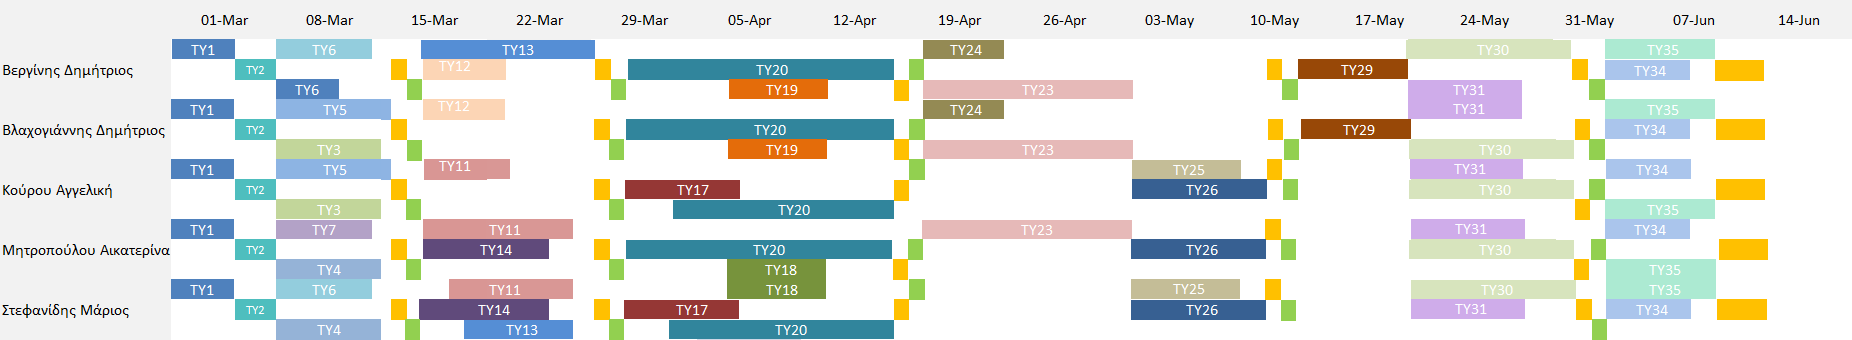
\includegraphics[width=1.0\textwidth]{HR Gantt Team Plan (Sceen).png}
\caption{\label{fig:HRGantt} HR Gantt Chart }
\end{figure}

\end{document}